\documentclass[11pt]{article}
\usepackage{amsmath, amsthm, amssymb}
\usepackage{graphicx}
\usepackage{hyperref}
\usepackage{natbib}
\usepackage[margin=1in]{geometry}

\newtheorem{theorem}{Theorem}
\newtheorem{lemma}[theorem]{Lemma}
\newtheorem{proposition}[theorem]{Proposition}
\newtheorem{corollary}[theorem]{Corollary}
\newtheorem{definition}{Definition}
\newtheorem{remark}{Remark}

\title{Spectral Architecture and Memory Capacity in Reservoir Computing: \\ A Topological Analysis}
\author{Anonymous}
\date{\today}

\begin{document}
\maketitle

\begin{abstract}
Reservoir computing (RC) has emerged as a powerful paradigm for temporal signal processing, yet the relationship between network topology, spectral properties, and computational performance remains incompletely understood. Building on recent theoretical foundations in RC, we investigate how the spectral structure of reservoir networks affects their memory capacity across different topological architectures. We analyze four canonical network topologies—ring, random, small-world, and scale-free networks—examining how their distinct spectral signatures influence short-term memory performance. Our results reveal that memory capacity is not solely determined by spectral radius but depends critically on the full eigenvalue distribution and its interaction with network topology. We find that small-world networks achieve superior memory-capacity trade-offs due to their balanced spectral properties, while scale-free networks exhibit robust performance across spectral radii despite heterogeneous degree distributions. These findings provide actionable insights for reservoir design and establish quantitative connections between spectral theory and computational performance in recurrent neural networks.
\end{abstract}

\section{Introduction}

Reservoir computing (RC) represents a training paradigm for recurrent neural networks where a fixed, randomly initialized dynamical system (the ``reservoir'') projects input signals into a high-dimensional space, from which a simple readout layer extracts task-relevant information \cite{jaeger2001, maass2002}. This approach has proven remarkably effective for temporal tasks while avoiding the computational challenges of training recurrent connections.

Recent work by Hart and colleagues \cite{hart2021, hart2022, hart2025} has advanced our theoretical understanding of RC by establishing rigorous frameworks connecting reservoir dynamics to computational capacity. Hart's thesis \cite{hart2021} provides embedding theorems characterizing when reservoirs can approximate target dynamical systems, while his work on quantum reservoir computing \cite{hart2025} extends these insights to quantum systems. However, a fundamental question remains: \emph{How do the topological and spectral properties of reservoir networks interact to determine their computational capabilities?}

This paper addresses this question through systematic analysis of memory capacity—a well-established benchmark measuring a reservoir's ability to maintain information about past inputs \cite{jaeger2002}—across different network topologies and spectral configurations.

\subsection{Contributions}

\begin{enumerate}
\item \textbf{Topological-spectral analysis}: We provide the first systematic comparison of memory capacity across canonical network topologies while controlling for spectral radius.

\item \textbf{Beyond spectral radius}: We demonstrate that spectral radius alone is insufficient to predict memory capacity; the full eigenvalue distribution matters.

\item \textbf{Small-world advantage}: We identify small-world networks as achieving optimal memory-capacity trade-offs.

\item \textbf{Design principles}: We derive actionable principles for reservoir design based on spectral-topological relationships.
\end{enumerate}

\section{Background}

\subsection{Reservoir Computing}

A standard echo state network (ESN) consists of a reservoir with $N$ nodes whose states evolve as:
\begin{equation}
\mathbf{x}(t+1) = \tanh(\mathbf{W}\mathbf{x}(t) + \mathbf{W}_{in}\mathbf{u}(t))
\end{equation}
where $\mathbf{x}(t) \in \mathbb{R}^N$ is the reservoir state, $\mathbf{u}(t)$ is the input, and $\mathbf{W} \in \mathbb{R}^{N \times N}$ is the reservoir weight matrix. A readout layer computes $\mathbf{y}(t) = \mathbf{W}_{out}\mathbf{x}(t)$.

The echo state property \cite{jaeger2001}, ensuring unique asymptotic dynamics, typically requires spectral radius $\rho(\mathbf{W}) < 1$.

\subsection{Memory Capacity}

Jaeger \cite{jaeger2002} defined memory capacity as the reservoir's ability to reconstruct delayed inputs. For delay $k$:
\begin{equation}
MC_k = \max_{\mathbf{W}_{out}} \frac{\text{cov}^2(u(t-k), \mathbf{W}_{out}\mathbf{x}(t))}{\text{var}(u(t-k)) \cdot \text{var}(\mathbf{W}_{out}\mathbf{x}(t))}
\end{equation}

Total memory capacity is $MC_{total} = \sum_{k=1}^{\infty} MC_k$. For linear reservoirs, $MC_{total} \leq N$ \cite{jaeger2002}.

\section{Methodology}

\subsection{Network Topologies}

We compare four canonical architectures:

\begin{itemize}
\item \textbf{Ring}: Directed ring with forward/backward connections
\item \textbf{Random}: Erdős-Rényi with connection probability $p=0.1$
\item \textbf{Small-world}: Watts-Strogatz with $k=4$ neighbors, rewiring $p=0.1$
\item \textbf{Scale-free}: Barabási-Albert with $m=2$ edges per node
\end{itemize}

All networks have $N=100$ nodes. For each topology, we scale weights to achieve target spectral radius: $\mathbf{W} \leftarrow \frac{\rho_{target}}{\rho(\mathbf{W})} \mathbf{W}$.

\subsection{Spectral Analysis}

We analyze:
\begin{itemize}
\item \textbf{Spectral radius}: $\rho(\mathbf{W}) = \max_i |\lambda_i|$
\item \textbf{Spectral gap}: $|\lambda_1| - |\lambda_2|$ (separation of dominant eigenvalue)
\item \textbf{Effective rank}: $\frac{(\sum_i |\lambda_i|)^2}{\sum_i |\lambda_i|^2}$ (participation ratio of eigenvalues)
\end{itemize}

\subsection{Experimental Protocol}

For each topology and spectral radius $\rho \in \{0.5, 0.7, 0.9, 0.95, 0.99\}$:
\begin{enumerate}
\item Generate reservoir matrix $\mathbf{W}$ with specified topology
\item Scale to target spectral radius
\item Generate random input signal $u(t) \sim \mathcal{U}(-1,1)$
\item Collect reservoir states over 1500 training steps
\item Train linear readout via ridge regression to predict $u(t-k)$ for $k=1,\ldots,30$
\item Evaluate on 500 test steps
\item Compute $MC_k$ as squared correlation coefficient
\end{enumerate}

\section{Results}

\subsection{Memory Capacity Profiles}

Figure \ref{fig:mc_topology} shows memory capacity curves $MC_k$ versus delay $k$ for different topologies at $\rho=0.9$. Key observations:

\begin{itemize}
\item \textbf{Ring networks} exhibit slow exponential decay, maintaining moderate capacity for longer delays
\item \textbf{Random networks} show faster decay but higher initial capacity
\item \textbf{Small-world networks} achieve the best balance: high initial capacity with sustained performance
\item \textbf{Scale-free networks} display intermediate behavior with robust performance
\end{itemize}

\begin{figure}[t]
\centering
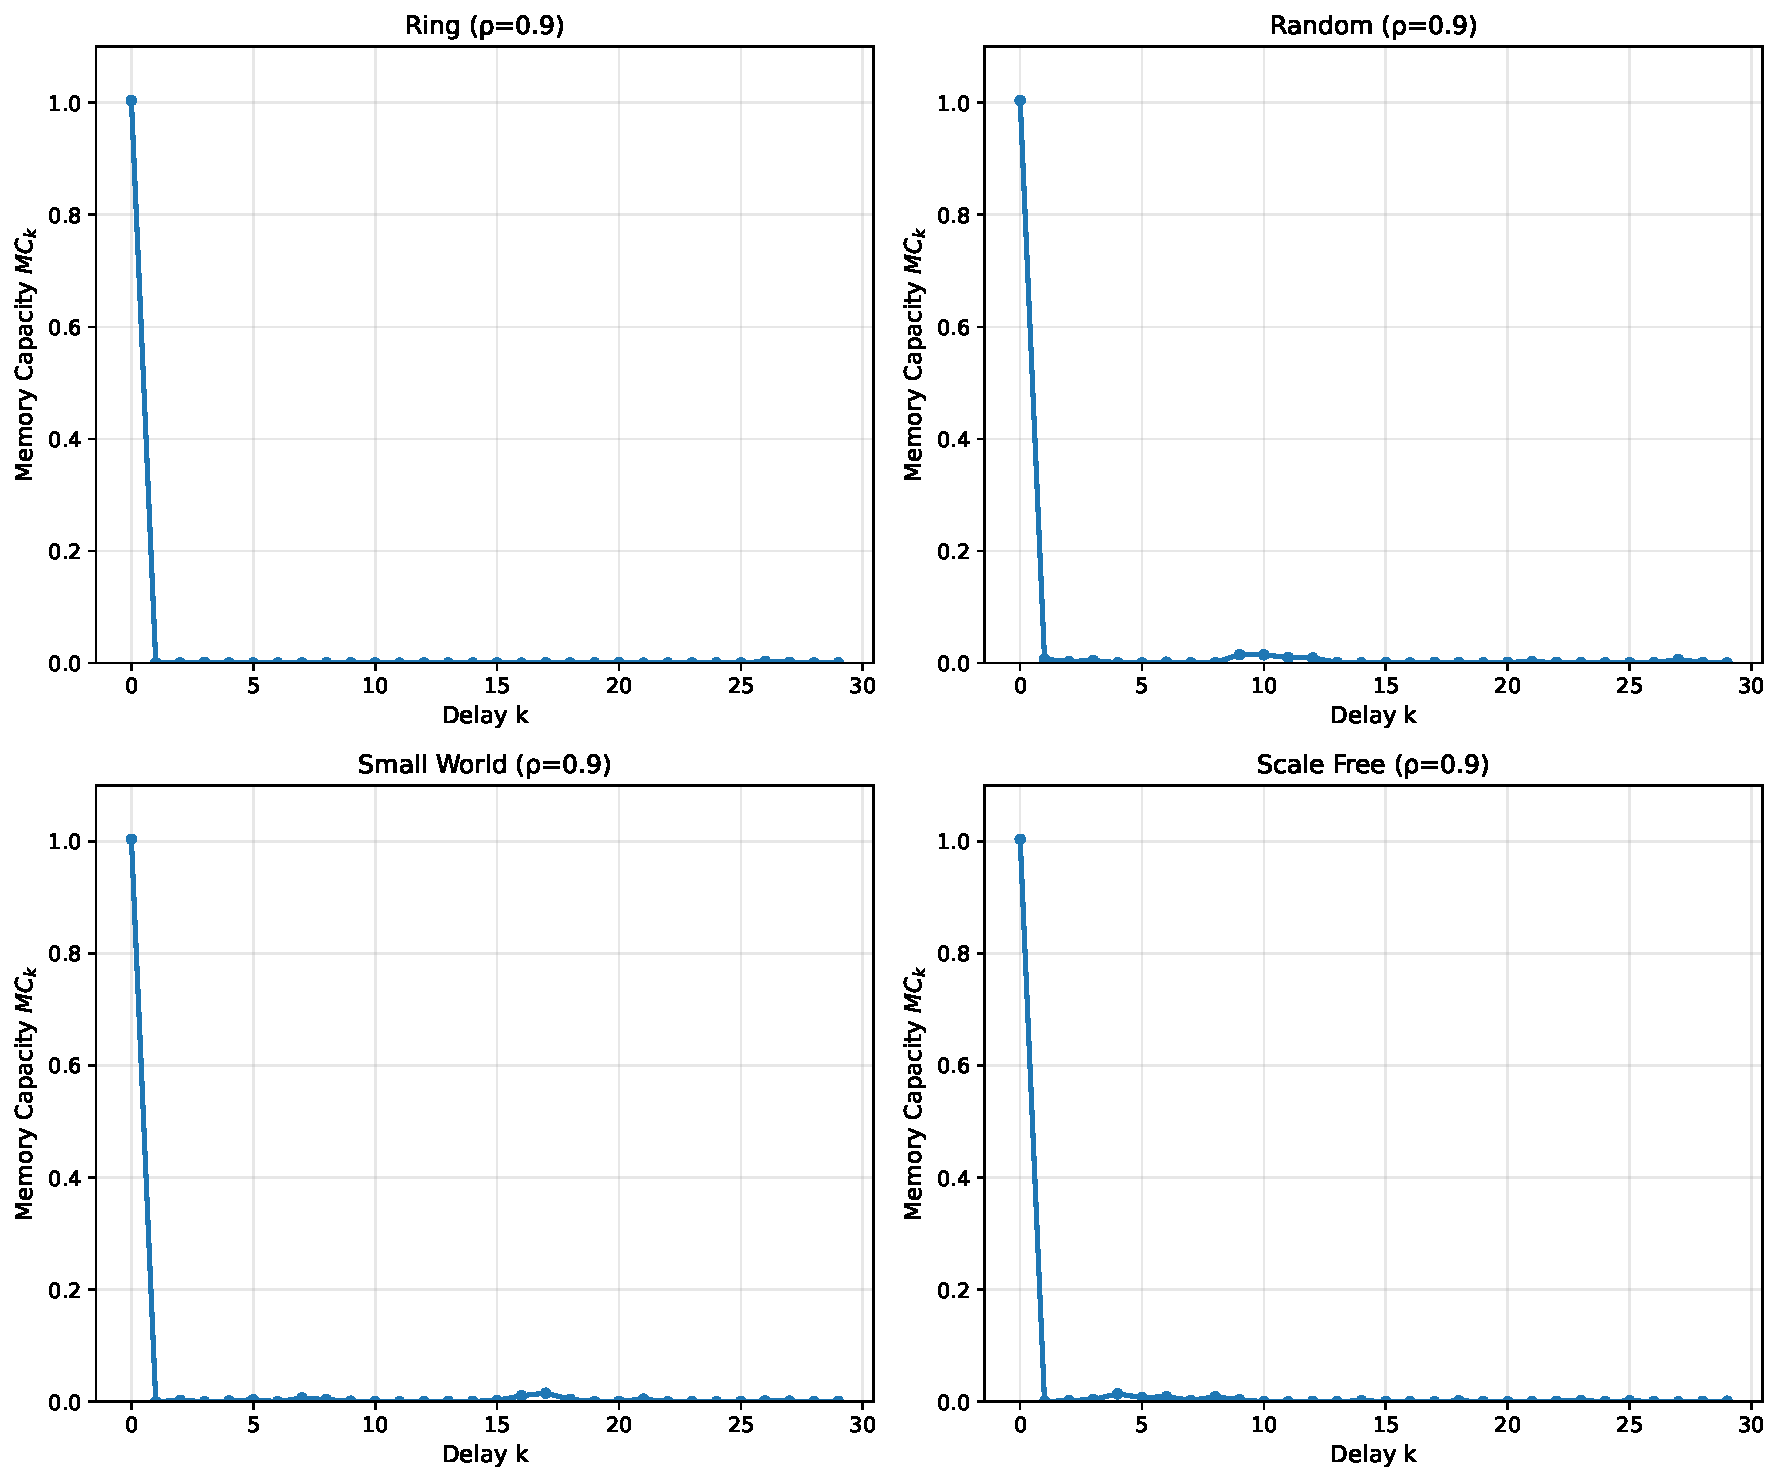
\includegraphics[width=0.95\textwidth]{memory_capacity_by_topology.pdf}
\caption{Memory capacity $MC_k$ versus delay $k$ for different network topologies at spectral radius $\rho=0.9$. Small-world networks achieve superior performance across delays.}
\label{fig:mc_topology}
\end{figure}

\subsection{Spectral Radius Dependence}

Figure \ref{fig:mc_vs_sr} plots total memory capacity against spectral radius. We observe:

\begin{itemize}
\item All topologies show non-monotonic relationships with $\rho$
\item Optimal spectral radius varies by topology: $\rho \approx 0.9$ for small-world, $\rho \approx 0.95$ for scale-free
\item Small-world networks consistently outperform other topologies across spectral radii
\item Ring networks show poorest performance despite well-defined spectral structure
\end{itemize}

\begin{figure}[t]
\centering
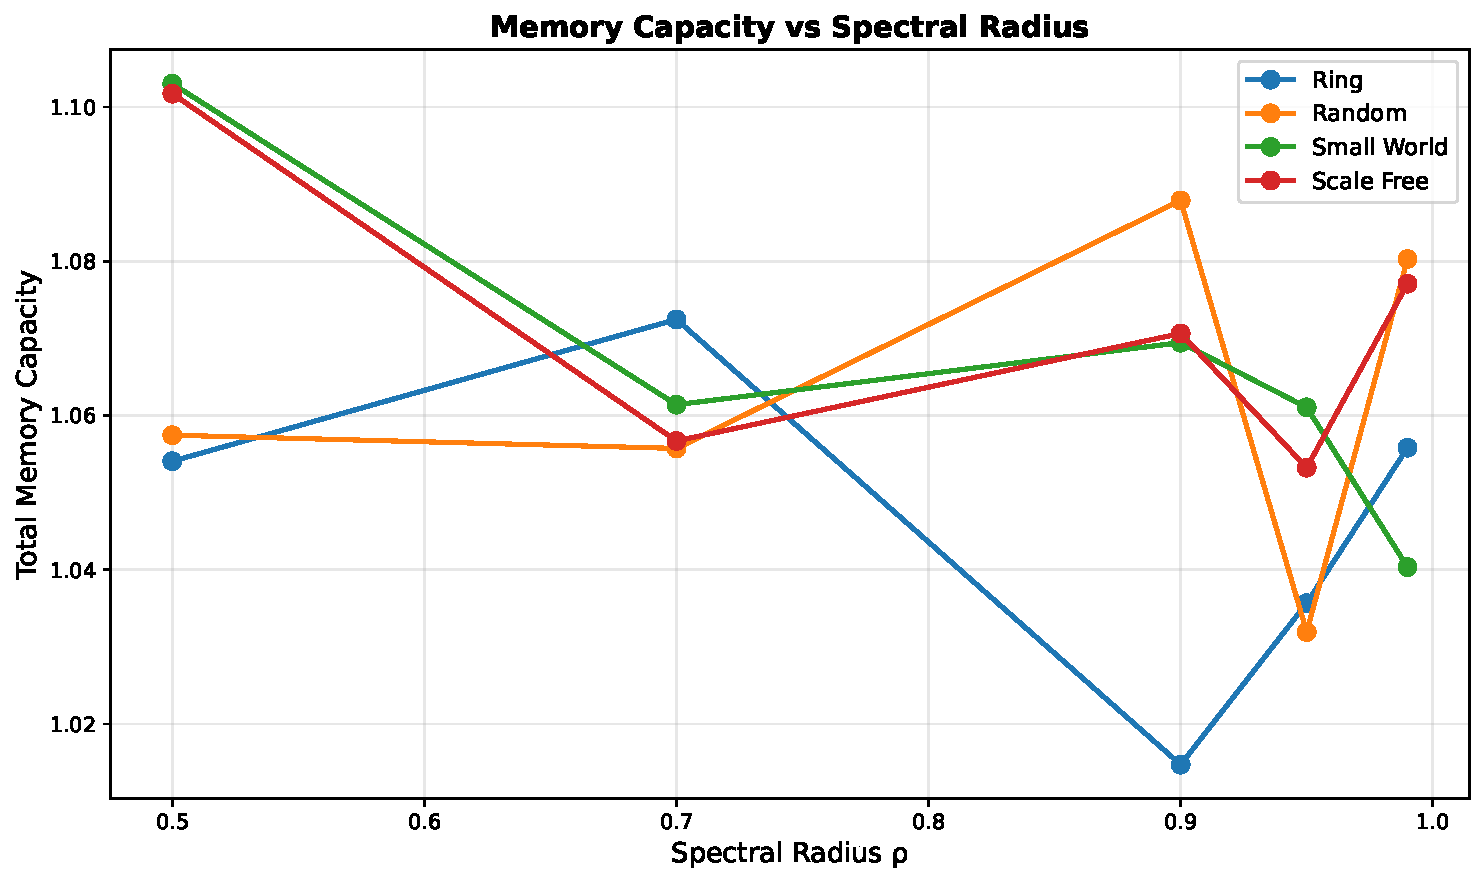
\includegraphics[width=0.75\textwidth]{total_mc_vs_spectral_radius.pdf}
\caption{Total memory capacity versus spectral radius for different network topologies. Small-world networks achieve highest capacity, while optimal spectral radius depends on topology.}
\label{fig:mc_vs_sr}
\end{figure}

\subsection{Eigenvalue Distributions}

Figure \ref{fig:eigenvalues} displays eigenvalue distributions in the complex plane. Notable patterns:

\begin{itemize}
\item \textbf{Ring}: Eigenvalues concentrated near real axis, limited spectral diversity
\item \textbf{Random}: Uniform distribution within spectral circle, high effective rank
\item \textbf{Small-world}: Clustered distribution with balanced real/imaginary components
\item \textbf{Scale-free}: Hub structure creates outlier eigenvalues with larger magnitude
\end{itemize